After a floor has been added we can add more objects to our world. We will start with agents.

\instruct{Create a new file agents.py}

As we are going to use functions (and classes) of the breve engine, we must import it at the top of our file.

\begin{lstlisting}[language=Python]
import breve
\end{lstlisting}

\instruct{Add the import statement to the top of our agents file.}

\section{Creating a simple agent}

We will start with a very simple agent which will do nothing but stand still. Every agent must extend the \textit{breve.Mobile} class in order for it to move and interact.

Just as with our controller, we have to add a constructor and an \textit{iterate} function.

\begin{lstlisting}[language=Python]
class SimpleAgent (breve.Mobile):

	def __init__(self):
		breve.Mobile.__init__(self)

		print "Created agent"

	def iterate(self):
		None
\end{lstlisting}

\instruct{Add the class definition above to the agents file.}

\instruct{Try to run the simulation and see what happens.}

As you can see nothing happened yet. This is because we still have to add our agent to the environment. This is done through the simulation controller.

\begin{lstlisting}[language=Python]
self.agent = agents.SimpleAgent()
\end{lstlisting}

\instruct{Add the snippet to the \textit{\_\_init\_\_} function of the controller, just below the lighting settings.}


\begin{figure}[htbp]
\begin{center}
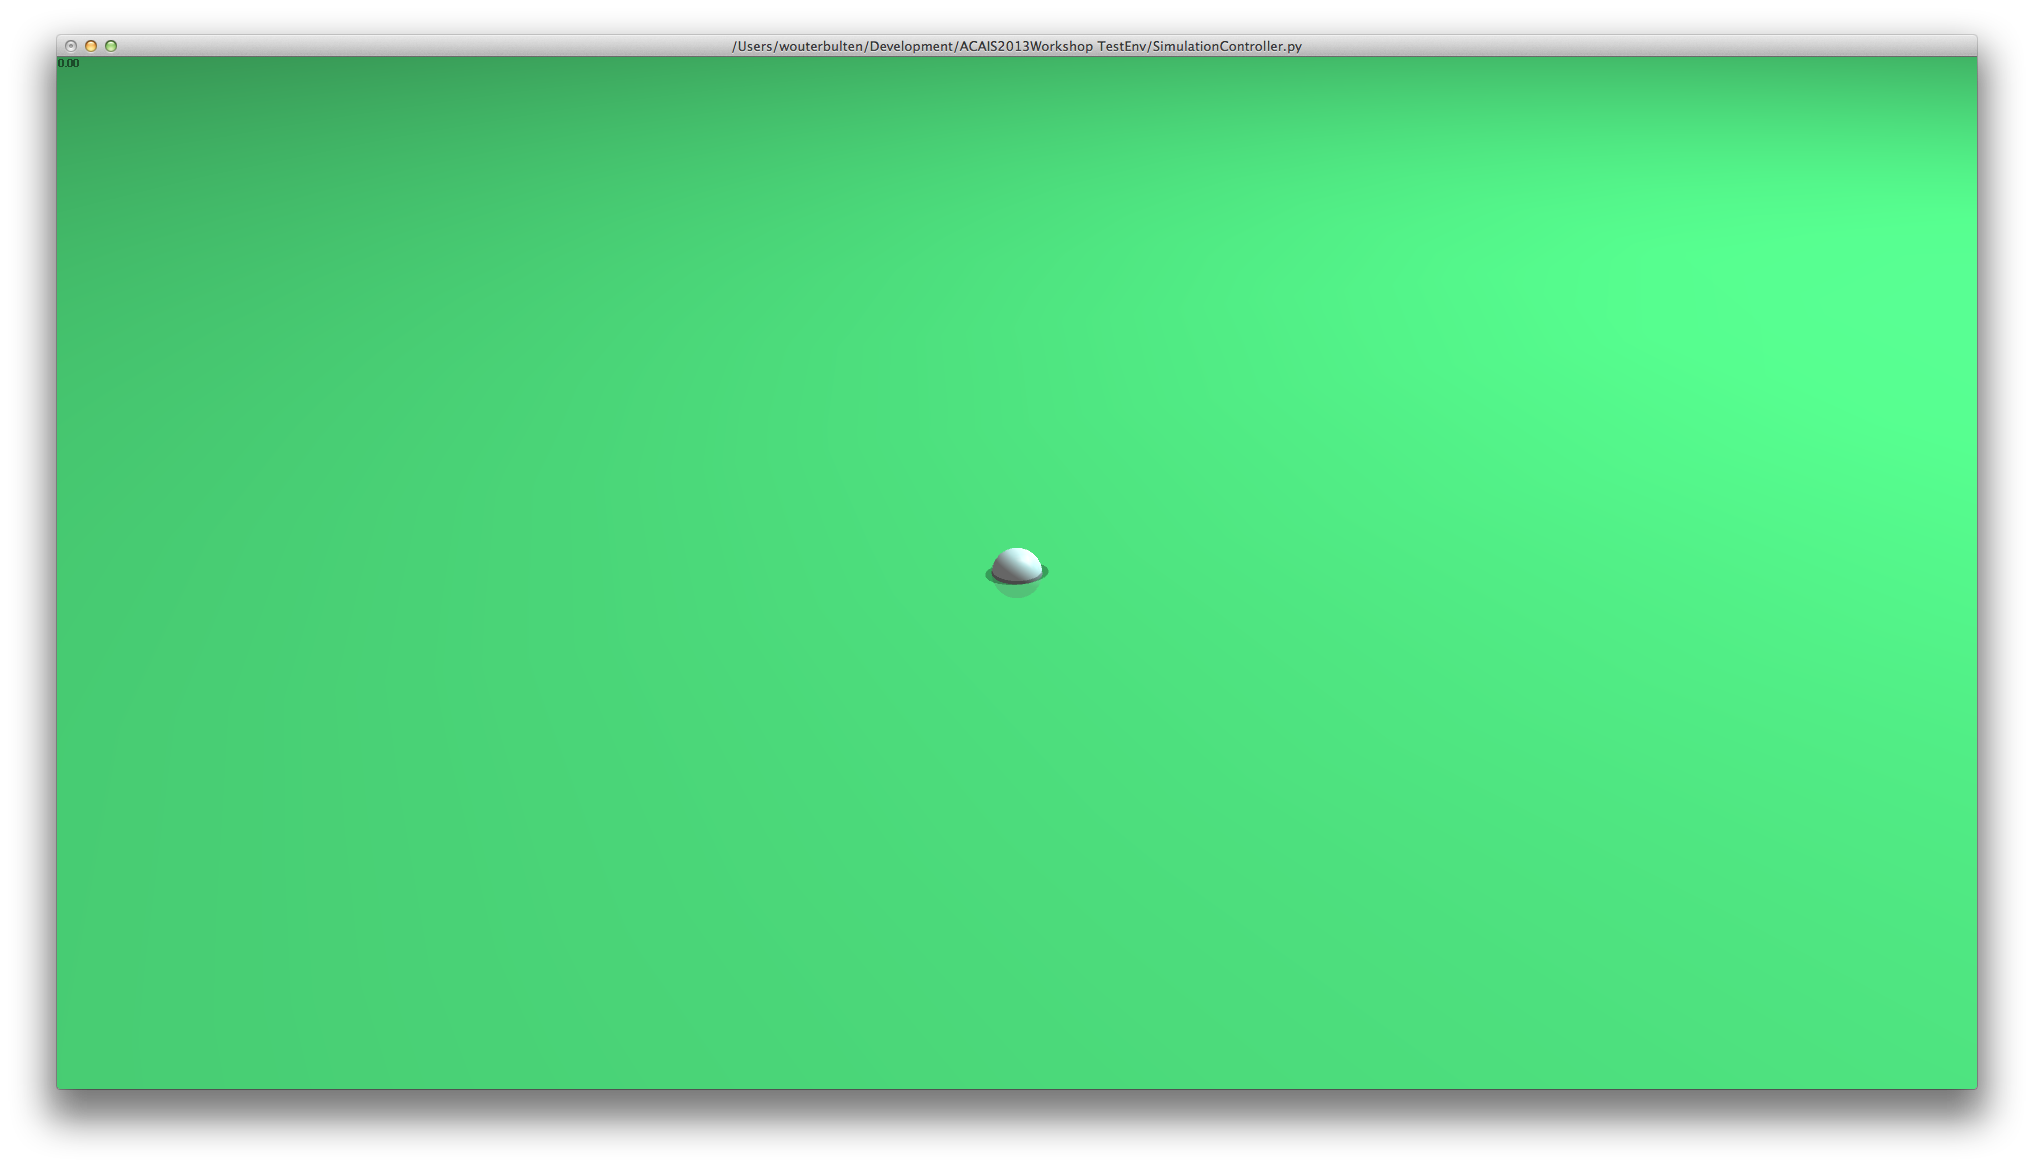
\includegraphics{graphics/simpleagent}
\caption{A single very simple agent has been added to the environment.}
\end{center}
\end{figure}

\section{Movement}
This agent is very boring, it just sits there and does nothing. We will create a new agent which wanders around in the world.

\begin{fullwidth}
\begin{lstlisting}[language=Python]
class RandomAgent (breve.Wanderer):
	def __init__(self):
		breve.Wanderer.__init__(self)

		self.setWanderRange(breve.vector(20, 0, 20))
		print "Created agent"

	def iterate(self):
		breve.Wanderer.iterate(self)
\end{lstlisting}
\end{fullwidth}

\instruct{Add the new agent class below the \textit{SimpleAgent}.}

This \textit{RandomAgent} extends the built in wanderer class of breve. The only setting we have to set is the range of the wanderer, in this case we set it to 20 in a 2D plane. It is important to call the super \textit{iterate} function, otherwise the wander behaviour will not be executed.

\section{Appearance}

Within Breve it is very easy to change the appearance of objects and agents. As an example we are going to change the shape of our agent to a cube. As we will add more agents in the future, we will define one shape object for all agents.

\instruct{Add the following to the constructor of the SimulationController:}
\begin{fullwidth}
\begin{lstlisting}[language=Python]
# Create a shape for the agents
self.agentShape = breve.createInstances(breve.Cube, 1).initWith(breve.vector(1,1,1))
\end{lstlisting}
\end{fullwidth}

This single line will create a cube with a dimension of 1x1x1. To be able to use this shape in our agent we add a getter method to the controller.

\instruct{Add the following getter to the simulation controller:}
\begin{lstlisting}[language=Python]
def getAgentShape(self):
	return self.agentShape
\end{lstlisting}

It is now very easy to change the shape of the agent. Every \textit{Real}\footnote{The Real object is a base class for more high-level classes such as Mobile and Stationary.} object within breve has access to the simulation controller using the variable \textit{controller}. We change the shape like so:

\begin{lstlisting}[language=Python]
# Set the shape of the agent
self.setShape(self.controller.getAgentShape())
\end{lstlisting}

\instruct{Try to change the shape of the agent by adding the code to the constructor of the agent. Test it by running the simulation, has the shape changed?}